Il processo di “\textit{Risk Management}” è l'insieme di attività coordinate
per gestire un'organizzazione con riferimento ai rischi.
Tipicamente include l'identificazione, la misurazione e la mitigazione delle
varie esposizioni al rischio.
Il rischio è l'incertezza che eventi inaspettati possano manifestarsi producendo
effetti negativi per l'organizzazione.
Il rischio di Information Technology è definito come il pericolo di interruzione
di servizio (\textit{availability}), diffusione di informazioni riservate
(\textit{riservatezza}) o di perdita di dati rilevanti
archiviati tramite mezzi computerizzati (\textit{integrità}).
Per operare su questi rischi è stata introdotta la
“\textit{Information Security Risk Management}”.
Va ricordato che Identificazione e Misurazione sono racchiusi nella
Risk Assessment.

\begin{figure}[H]
    \centering
    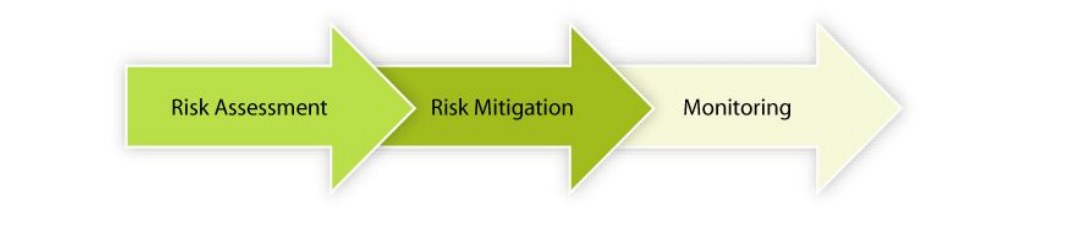
\includegraphics[width=12cm, keepaspectratio]{capitoli/risks/imgs/risk1.png}
\end{figure}